\documentclass[twocolumn]{aastex701}

\journalinfo{}
\makeatletter
\renewcommand{\frontmatter@title@above}{}
\makeatother
\AtBeginDocument{\hypersetup{colorlinks=true,linkcolor=black,citecolor=xlinkcolor,urlcolor=xlinkcolor,filecolor=black}}
\shorttitle{Testing Baryonic Geometric-Response Information}
\shortauthors{}
 

% Local production preview style: suppress running heads and place page numbers
% at the bottom center. AAS production will apply the final published style.
\makeatletter
\def\ps@apjheads{%
  \let\@mkboth\@gobbletwo
  \let\@oddhead\@empty
  \let\@evenhead\@empty
  \def\@oddfoot{\hfil\thepage\hfil}%
  \def\@evenfoot{\hfil\thepage\hfil}%
}
\def\ps@plain{%
  \let\@mkboth\@gobbletwo
  \let\@oddhead\@empty
  \let\@evenhead\@empty
  \def\@oddfoot{\hfil\thepage\hfil}%
  \def\@evenfoot{\hfil\thepage\hfil}%
}
\def\ps@titlepage{%
  \let\@mkboth\@gobbletwo
  \let\@oddhead\@empty
  \let\@evenhead\@empty
  \def\@oddfoot{\hfil\thepage\hfil}%
  \def\@evenfoot{\hfil\thepage\hfil}%
}
\makeatother
\pagestyle{plain}

\begin{document}
\pagestyle{plain}

 \title{Testing Baryonic Geometric-Response Information on SPARC Rotation Curves}
 \author{Mohammed Messaoudene}
\altaffiliation{Corresponding author: Mohammed Messaoudene; email: \href{mailto:mohammed.messaoudene@univ-temouchent.edu.dz}{mohammed.messaoudene@univ-temouchent.edu.dz}; ORCID iD: \href{https://orcid.org/0009-0007-4665-2548}{0009-0007-4665-2548}.}
 \affiliation{Faculty of Sciences, Belhadj Bouchaib University of Ain Temouchent, Route of Sidi Bel Abbes, BP 284, 46000 Ain Temouchent, Algeria}
\email{mohammed.messaoudene@univ-temouchent.edu.dz}
 \correspondingauthor{Mohammed Messaoudene}
\begin{abstract}
We test whether baryonic geometric-response invariants add predictive information beyond a simple globally fitted square-root response on SPARC rotation curves. The fixed Geometric-Medium Response (GMR) prescription is evaluated on the 175-galaxy SPARC sample and on a held-out 151-galaxy subset with no galaxy-by-galaxy retuning. The central result is a constraint rather than a superiority claim: a pure $\sqrt{g_N}$ control reaches slightly lower equal-weight RMSE than full GMR on both the full and held-out samples (40.241/41.329 versus 40.554/41.870 km\,s$^{-1}$). Thus the tested baryonic-invariant architecture does not improve the main aggregate RMSE benchmark beyond the simpler square-root scaling. GMR remains competitive relative to baryons-only, MOND, and reduced NFW on the same aggregate metric, but reduced NFW retains the smaller median residual and higher per-galaxy win rate, while reduced ISO and Burkert remain stronger empirical halo prescriptions overall. A local-$S_\Psi$ replacement performs worse than the cumulative-state GMR implementation, so the cumulative state variable is useful relative to that ablation even though the full invariant structure is not empirically necessary on the primary RMSE metric. The main empirical failure mode remains the low-mass, low-surface-brightness dwarf regime. The contribution is therefore a reproducible constraint on the utility of the tested geometric invariants for SPARC rotation curves, not a demonstration that full GMR is a superior fitting model. Screening, cosmological perturbations, clusters, strong-field behavior, dark-energy closure, vector response, external-field geometry, and dwarf-spheroidal systems are not tested here.
\end{abstract}
 \keywords{Galaxy rotation curves (619) --- Disk galaxies (391) --- Dwarf galaxies (416) --- Low surface brightness galaxies (940) --- Dark matter (353) --- Astrostatistics (1882)}

\section{Introduction}

Galaxy rotation curves remain one of the cleanest empirical tests of how much information about the missing-mass phenomenology is already carried by the baryonic field. In the contemporary literature, that test is usually organized around baryons-only baselines, modified-gravity relations such as MOND, and flexible halo fits such as NFW or cored empirical alternatives. The SPARC compilation sharpened the comparison by assembling 175 nearby disk galaxies with homogeneous 3.6 micron photometry, resolved rotation curves, and public mass-model products \citep{lelli2016}. The same sample also underlies the modern radial-acceleration relation (RAR) and baryonic Tully-Fisher relation (BTFR) literature \citep{mcgaugh2016,lelli2019}. The comparison families connect to classic rotation-curve evidence \citep{rubin1980}, MOND phenomenology \citep{milgrom1983,famaey2012}, and standard halo profiles \citep{navarro1997,burkert1995}.

This study asks a narrower and more falsifiable question than the broader theoretical program would imply. We treat the Geometric-Medium Response (GMR) model as a fixed galaxy phenomenology and ask whether its baryonic geometric invariants add predictive information beyond a simple square-root response once the benchmark, comparator set, and reporting rules are fixed in advance. The analysis does not present a total dark-sector theory, an action principle, or a precision-cosmology completion.

This work is restricted to galaxy-scale SPARC phenomenology. Screening, cosmological perturbations, clusters, strong-field behavior, and dark-energy closure are not tested here and are left for future work. Extensions involving vector response, external-field geometry, or dwarf-spheroidal systems are not tested here and remain future work.

Within that scope, the fixed implementation remains worth reporting because it provides a controlled constraint on the geometric-response idea. On the full 175-galaxy benchmark GMR reaches an equal-weight RMSE of 40.554 km\,s$^{-1}$, compared with 40.241 for the pure square-root control, 69.316 for baryons, 44.907 for MOND, and 46.613 for reduced NFW. On the held-out 151-galaxy subset the corresponding values are 41.870, 41.329, 71.026, 45.366, and 48.450 km\,s$^{-1}$. The dominant SPARC aggregate signal is already captured by square-root scaling; the tested GMR invariant architecture organizes geometric departures from that scaling but does not improve the main RMSE benchmark.

The analysis reports the aggregate equal-weight RMSE, complementary descriptive diagnostics, and explicit failure modes across galaxy classes. Relation-level diagnostics are used within their stated scope: the RAR as a within-sample consistency test and the BTFR as a supportive but imperfect scaling-law check. The main empirical limitation of the present implementation occurs in low-mass, low-surface-brightness dwarf systems, where reduced halo fits retain a strong pointwise advantage.

That limitation is also the clearest falsifiability handle. Within the present scope, the fixed implementation would be challenged if independent dwarf-dominated low-surface-brightness samples reproduce the same level of local failure while the claimed aggregate non-dwarf SPARC advantage does not persist under the same fixed parameters. The analysis is written to make that narrow empirical status explicit.

The surrounding literature sets the empirical and methodological context. Classical rotation-curve and distance-scale context comes from disk and dark-halo work \citep{freeman1970,tully1977,rubin1978,rubin1980,bosma1981,begeman1991,sofue2001}. The SPARC, RAR, and BTFR comparisons sit within the modern empirical scaling-relation literature \citep{lelli2016,mcgaugh2016,lelli2019,mcgaugh2000,mcgaugh2005,mcgaugh2012,stark2009}. MOND and relativistic modified-gravity work provide phenomenological context without being treated here as closed alternatives \citep{milgrom1983,sanders2002,famaey2012,bekenstein2004,skordis2021,milgrom2014}. The halo baselines and failure modes are interpreted against standard CDM, cored-profile, and small-scale-structure discussions \citep{navarro1997,burkert1995,deblok2001,deblok2008,moore1999,boylankolchin2011,bullock2017,pontzen2012,governato2012,dicintio2014,oman2015,sales2017,maccio2008,dutton2014,planck2020}. Stellar mass-to-light and dwarf-galaxy systematics are also relevant for the limited empirical interpretation \citep{chabrier2003,bell2003,meidt2014,oh2015}. Medium-like and emergent dark-sector analogies are only background motivation \citep{berezhiani2015,verlinde2017}. The statistical and software stack follows standard bootstrap, multiple-testing, effect-size, and scientific-Python references \citep{efron1979,efron1987,wilson1927,cohen1988,holm1979,hunter2007,harris2020,virtanen2020,reback2020}.

\section{Geometric-medium response framework}

GMR is treated here as a fixed phenomenological response closure rather than as a completed fundamental theory. The motivating picture is that baryons source not only the directly computed Newtonian field but also a structured medium response, but the present article does not claim an action principle or a unique microscopic derivation. The model is applied using a fixed prescription: a single architecture with the same global parameters is used for all galaxies, with no galaxy-by-galaxy retuning.

That fixed-implementation protocol is what turns the SPARC test into something more than a flexible interpolation exercise. A fixed implementation can be used to test whether geometric baryonic invariants add information beyond a simpler response law, whereas a flexible family can absorb local failures by changing knobs object by object. At the same time, the analysis does not imply that universality alone confers superiority. Reduced halo fits buy local precision through per-galaxy flexibility, while GMR pays for fixed global response with weaker local adaptability. The correct interpretation is therefore a global-response-versus-flexibility comparison, not a parameter-parity contest.

That narrower scope follows directly from that logic. Earlier iterations of the broader research program sometimes carried screening or backend notes alongside the galaxy analysis because those sectors existed elsewhere in the analysis products. The present analysis does not use them as evidence. The result being claimed here is a fixed galaxy phenomenology on SPARC, plus relation-level and robustness diagnostics drawn from the same machine-readable analysis tables.

That narrower presentation makes the empirical claim more precise. If the geometric terms add predictive power under those conditions, then the analysis would support the extra invariant structure. If the simpler square-root control already captures the dominant aggregate signal, that limitation is also a concrete result. Both are empirical results; neither implies that the larger geometric program is already closed.
\section{Fixed GMR model and equations}

The public Geometric-Medium Response (GMR) model used in this paper corresponds to a stored implementation carried into the SPARC analysis tables. The galaxy-level prediction is therefore reconstructed from the stored implementation and from the fixed parameter tables used to generate the final figures and metrics reported here.


\subsection{Motivation of the GMR invariants}

The fixed prescription uses the baryonic field as a set of local and non-local diagnostics rather than as a derivation from a completed action. The quantity $A_B$ is used as a local baryonic amplitude invariant, measuring the relative strength of the trace-free tidal structure against the scalar baryonic source term. The compactness variable $C_B$ is a curvature/compactness diagnostic that compares the local baryonic curvature scale with the radial-field scale. The bounded combination $\nu_B$ acts as a local structural-regime tracer, while $S_\Psi$ accumulates that tracer across radius and therefore supplies the non-local state variable used by the response law.

In this prescription, $\alpha_B$ is an effective response angle: it maps the local baryonic invariants and the cumulative state variable into a bounded orientation-like response. The acceleration $g_\chi$ is then the effective geometric-response acceleration added to the Newtonian baryonic acceleration. The factor $S_{\rm rad}$ is only a phenomenological radial suppression factor in the galaxy-scale prescription; it is not used here as evidence for local Solar-System screening. The baryonic input is the SPARC midplane Newtonian acceleration $g_N(R)$ imported from the stored source record for each galaxy. The corresponding baryonic circular speed is
\begin{equation}
v_{\rm bar}(R) = \frac{\sqrt{R\,g_N(R)}}{10^3},
\end{equation}
with $R$ in meters and $v_{\rm bar}$ reported in km\,s$^{-1}$. On the baryonic source grid, the implementation solves the axisymmetric Poisson problem
\begin{equation}
\nabla^2 \phi_B = 4\pi G\rho_b,
\end{equation}
and constructs the baryonic invariants
\begin{equation}
T_{ii} = \phi_{ii} - \frac{1}{3}\nabla^2\phi_B,
\qquad
\|T\| = \sqrt{T_{RR}^2 + T_{\phi\phi}^2 + T_{zz}^2},
\end{equation}
\begin{equation}
A_B(R) = \frac{\|T(R)\|}{|\nabla^2\phi_B(R)| + \epsilon},
\end{equation}
\begin{equation}
C_B(R) = \frac{\ell_*\,|\nabla^2\phi_B(R)|}{\sqrt{(\partial_R \phi_B)^2 + A_*^2 + \epsilon}},
\end{equation}
together with
\begin{equation}
\nu_B(R) = \frac{A_B(R) + C_B(R)}{1 + A_B(R) + C_B(R)}.
\end{equation}

The selected fixed state variable is the current-cumulative proxy. In the stored implementation it is evaluated on the observed radial grid as
\begin{equation}
Q_{\rm enc}(R_i) = \sum_{j\le i} \nu_B(R_j)\,\Delta R_j,
\end{equation}
\begin{equation}
S_\Psi(R_i) = \frac{Q_{\rm enc}(R_i)}{Q_* + Q_{\rm enc}(R_i)}.
\end{equation}

The fixed alignment closure is the additive-saturation form
\begin{equation}
\alpha_B(R_i) = \arctan\left[\frac{A_B(R_i) + \eta_S S_\Psi(R_i)}{1 + C_B(R_i)}\right].
\end{equation}

The internal radial suppression factor used by the fixed galaxy phenomenology is
\begin{equation}
S_{\rm rad}(R_i) = \left[1 + \lambda_s\,\nu_B(R_i)\,C_B(R_i)\right]^{-1}.
\end{equation}

The scalar-response acceleration and final circular-speed prediction are
\begin{equation}
g_\chi(R_i) = \mathcal{A}_{\rm GMR}\,\sin\alpha_B(R_i)\,\sqrt{g_N(R_i)}\,S_{\rm rad}(R_i),
\end{equation}
\begin{equation}
g_{\rm tot}(R_i) = g_N(R_i) + g_\chi(R_i),
\end{equation}
\begin{equation}
v_{\rm GMR}(R_i) = \frac{\sqrt{R_i g_{\rm tot}(R_i)}}{10^3}.
\end{equation}

All galaxies are evaluated with the same fixed global values: $A_* = 10^{-10}\,{\rm m\,s^{-2}}$, $\ell_* = 1\,{\rm kpc}$, $Q_* = 10^{20}\,{\rm m}$, $\eta_S = 6.0$, $\mathcal{A}_{\rm GMR} \approx 1.395\times10^{-5}\,(\mathrm{m\,s^{-2}})^{1/2}$, $\lambda_s = 10.0$, and numerical regularizer $\epsilon = 10^{-30}$ in the displayed invariant denominators.

The regularizer is applied in the normalized denominator units of the invariant construction. It is a dimensionless numerical floor in those normalized code units, not an additional physical acceleration scale.

These equations define the fixed phenomenological prescription tested here; they are not claimed in this paper to follow from a closed relativistic action.


\begin{table*}[t]
\centering
\scriptsize
\setlength{\tabcolsep}{3pt}
\caption{Parameter provenance for the fixed SPARC phenomenology. The optimized global response parameters are $\mathcal{A}_{\rm GMR}$ and $\lambda_s$. The remaining constants are fixed structural scales or numerical regularizers used by the tested prescription and are treated as effective model complexity rather than cost-free assumptions.}
\begin{tabular*}{\textwidth}{@{\extracolsep{\fill}}llllll}
\hline
Symbol & Value & Role & Optimized/fixed & Provenance & Sensitivity status \\
\hline
$\mathcal{A}_{\rm GMR}$ & $1.3946\times10^{-5}$ & response amp. & optimized & calibration\_24 grid & BCa/RMSE \\
$\lambda_s$ & 10.0 & suppression strength & optimized & calibration\_24 grid & BCa/RMSE \\
$A_*$ & $10^{-10}$ m s$^{-2}$ & accel. scale & fixed & stored prescription & complexity count \\
$\ell_*$ & 1 kpc & length scale & fixed & stored prescription & complexity count \\
$Q_*$ & $10^{20}$ m & state scale & fixed & stored prescription & complexity count \\
$\eta_S$ & 6.0 & state gain & fixed & stored prescription & complexity count \\
$\epsilon$ & $10^{-30}$ & denominator floor & fixed & numerical floor & not physical \\
\hline
\end{tabular*}
\end{table*}

The response amplitude also defines the acceleration scale $\mathcal{A}_{\rm GMR}^2 = 1.945\times10^{-10}\,{\rm m\,s^{-2}}$, within a factor of 1.62 of Milgrom's canonical $a_0$. This proximity is an empirical scale coincidence of the fixed SPARC phenomenology, not an imposed equality or an independent derivation of MOND.

\subsection{Relation to MOND-like square-root scaling}

The response law contains a factor $g_\chi\propto \sqrt{g_N}$, so it deliberately overlaps with the square-root scaling that appears in the deep-MOND acceleration excess. This similarity is part of the reason the response scale $\mathcal{A}_{\rm GMR}^2=1.945\times10^{-10}\,{\rm m\,s^{-2}}$ is reported explicitly: it is close to, but not identified with, Milgrom's canonical $a_0$. In this paper that proximity is treated only as an empirical scale coincidence of the fixed SPARC phenomenology.

The fixed GMR equations differ formally from a pure MOND-like square-root law through the factor $\sin\alpha_B(R)S_{\rm rad}(R)$ and through the baryonic-invariant construction entering $\alpha_B$ and $S_{\rm rad}$. A recovered 3391-point radial diagnostic confirms that this factor is not constant: its median is 0.599, with a 5--95 percentile range of 0.063--0.967. However, a pure globally fitted $\sqrt{g_N}$ baseline optimized on the same calibration subset gives a full-sample equal-weight RMSE of 40.241 km\,s$^{-1}$, slightly below the recovered GMR value of 40.554 km\,s$^{-1}$. The present data therefore do not establish that the full baryonic-invariant response improves on the simpler square-root baseline. The comparison with MOND and square-root response laws is retained as a descriptive, metric-dependent diagnostic rather than a decisive distinctiveness claim.

The state variable is non-local in radius through the cumulative $Q_{\rm enc}(R_i)$ sum. A local relativistic Lagrangian realization, if developed in future work, would therefore require additional fields or an equivalent non-local representation.


The exact stored machine value of the response amplitude is retained for reproducibility in the supplement and parameter table: $\mathcal{A}_{\rm GMR} = 1.3945832491957465\times10^{-5}\,(\mathrm{m\,s^{-2}})^{1/2}$. In the calibration record, that amplitude is the fixed result of a global grid search over $(\mathcal{A}_{\rm GMR}, \lambda_s)$ on the calibration subset labeled \texttt{calibration\_24}, using equal-weight RMSE as the selection loss. The public manuscript rounds the amplitude because the phenomenological claim does not depend on optimizer-level significant digits; the exact stored value is kept only in the reproducibility record.

This also explains why the parameter table mixes rounded and exact-looking numbers. $Q_*$, $\eta_S$, and $\lambda_s$ are implementation-level structural scales retained in coarse or discrete form, whereas $\mathcal{A}_{\rm GMR}$ is the optimizer-selected global amplitude exported exactly from the archive. No galaxy-by-galaxy fit parameter enters the public prediction.

This analysis adds a conservative method-sensitivity interpretation of those constants. The structural scales $A_*$, $\ell_*$, $Q_*$, $\eta_S$, and $\epsilon$ are disclosed as fixed components of the tested prescription; their deeper calibration is not claimed to be statistically independent in this paper. For this reason the supplement reports AIC/BIC-like diagnostics both for the two optimized response parameters and for a conservative seven-constant effective-count interpretation. The available analysis artifact set does not contain a fully rerunnable all-constant SPARC sensitivity harness, so no stronger hyperparameter-robustness claim is made.
\section{Fixed implementation and allowed scope}

The implementation documented here is the fixed GMR prescription used throughout the SPARC analysis products. The fixed-implementation rule means that the equations, the fixed global parameters, the archived figure-source CSVs, and the machine-readable comparison tables are inherited unchanged from the fixed GMR prescription. The per-galaxy metrics table confirms that all 175 galaxies are evaluated with identical global parameters rather than hidden object-level knobs.

The scope of the empirical result is therefore limited to the galaxy-scale SPARC phenomenology tested here. GMR is not presented as ``the best model'' and not as a closed dark-sector theory. The reported result is that the fixed implementation improves over baryons-only, MOND, and reduced NFW on the aggregate equal-weight RMSE benchmark, while reduced NFW remains better on median residual and win rate and reduced ISO/Burkert remain stronger empirical halo prescriptions overall.

This work is restricted to galaxy-scale SPARC phenomenology. Screening, cosmological perturbations, clusters, strong-field behavior, and dark-energy closure are not tested here and are left for future work. Extensions involving vector response, external-field geometry, or dwarf-spheroidal systems are not tested here and remain future work.

The phrase ``reduced'' is also fixed operationally in this paper. Reduced NFW, reduced ISO, and reduced Burkert denote the archived per-galaxy two-parameter halo baselines already exported in the fixed tables. By contrast, baryons-only carries no dark-sector fit freedom, MOND is the single-global-constant comparison already used in the archived analysis, and GMR uses one fixed architecture with global parameters shared across the sample. The comparison is therefore informative, but it is not a claim of equal flexibility. In round numbers, the GMR prediction uses a globally fixed response prescription after the implementation is fixed, while the reduced halo baselines carry two halo parameters for each galaxy, or approximately 350 halo degrees of freedom across the full 175-galaxy sample.

The analysis is therefore limited to a reproducible SPARC rotation-curve phenomenology with explicit failure modes, relation-level consistency checks, and reproducibility artifacts. No broader claim is made in this work.
\section{SPARC data and baseline models}

The galaxy benchmark is the official SPARC sample \citep{lelli2016}, used here as a fixed set of 175 galaxies with public mass-model products and a machine-readable per-galaxy summary table. The analysis uses the same full sample and the same held-out subset throughout. The held-out subset contains 151 galaxies relative to the final two-parameter calibration, but it is not claimed to be an independently preregistered data set. The full machine-readable table contains 175 galaxies. The sample accounting report also tracks 3391 mass-model rows.

A practical issue for figure design is the uneven information content across galaxies. Four objects have fewer than five observed rotation-curve points, and 32 have fewer than eight. The main-text atlas therefore obeys a hard rule: galaxies with fewer than eight observed points are excluded from the principal visual figure and retained only in the supplementary atlas. This is a presentation safeguard, not a hidden sample cut.

The calibration subset used for the final two-parameter calibration is listed explicitly in the supplement and in \texttt{tables/calibration\_24\_subset.csv}; it contains 24 named galaxies with class, surface-brightness proxy, gas-fraction proxy, and sampling information. The comparator set is fixed and operationally defined. Baryons-only is the zero-extra-flexibility baseline. MOND is the single-global-constant comparison already exported in the archived analysis. Reduced NFW, reduced ISO, and reduced Burkert are the archived per-galaxy halo baselines used in the same machine-readable tables. In this manuscript they are used only through the archived rotation-curve and residual columns: the article does not reconstruct a new halo fit and does not claim parameter-parity with flexible halo modelling. Where the older solver exports explicit reduced-halo parameters, the reduced ISO baseline is a two-parameter core-radius/velocity-scale fit; the NFW and Burkert baselines are treated here as archived per-galaxy reduced halo comparisons. Their inclusion matters because it prevents the paper from confusing a global response with blanket superiority; reduced ISO and Burkert remain stronger empirical halo prescriptions on aggregate.

A matched global-halo baseline is not implemented in this paper. That absence is a limitation: the reduced halo tables are descriptive empirical comparators, not an equal-parameter proof that GMR is superior to dark-matter prescriptions generally. A matched global-halo baseline, such as an NFW concentration--mass scaling relation or another low-dimensional halo scaling prescription, is not implemented here and remains an important next comparator. Therefore, the present results should not be read as broad superiority over dark-matter halo prescriptions generally.

The analysis conditions on the published SPARC distances, inclinations, and mass-model velocities. Distance, inclination, stellar mass-to-light, and covariance uncertainties are not fully propagated through the GMR comparison in this paper; the reported metrics should therefore be read as conditional on the archived SPARC kinematic and baryonic products.

The relation-level diagnostics are drawn from the same machine-readable table hierarchy. The RAR and BTFR results reported here come from machine-readable archived products and figure-source CSVs already present in the SPARC analysis. The methods section records that source hierarchy: it is an archived table synthesis built on fixed SPARC products, not a fresh upstream reprocessing of every raw SPARC product.

\begin{deluxetable}{ll}
\tablecaption{Sample accounting carried into the present analysis.}
\tablehead{\colhead{Quantity} & \colhead{Value}}
\startdata
Full SPARC sample galaxies & 175 \\
Held-out fixed subset galaxies & 151 \\
Mass-model rows & 3391 \\
Galaxies with $N_{\rm obs}<5$ & 4 \\
Galaxies with $N_{\rm obs}<8$ & 32 \\
Main-text visual rule & Exclude galaxies with $N_{\rm obs}<8$ \\
\enddata
\end{deluxetable}
\section{Statistical protocol and metric definitions}

The statistical protocol is designed to block the most common presentation failure in galaxy-fit papers: turning a one-metric advantage into a general superiority claim. Every principal comparison is therefore reported through four quantities whenever the machine-readable tables provide them: equal-weight RMSE across galaxies, mean absolute residual, median absolute residual, and per-galaxy win rate. Equal-weight RMSE remains the headline metric because it was the primary aggregate endpoint used for the fixed GMR prescription, but it is embedded in wider tabulated diagnostics so that a reader cannot miss when another comparator wins on a different notion of fit quality.

The model comparisons are reported as descriptive performance diagnostics rather than as family-wise significant inferential claims. Under a joint Holm-Bonferroni correction across the four RMSE contrasts, no contrast remains below $\alpha=0.05$. The held-out equal-weight RMSE is reported as the main descriptive aggregate metric. Mean, median, win rate, RAR, BTFR, and stratified diagnostics are reported as descriptive quantities.

Equal-weight RMSE is computed by treating each galaxy-level RMSE as one terminal observation and then taking the root-mean-square across galaxies. That makes it a natural global-response metric for a model that is fixed across heterogeneous disks. Its limitation is equally clear: it can reward a model that reduces the tail of catastrophic failures without necessarily improving the median galaxy. Unless otherwise stated, the median residual values reported in the aggregate comparison table are the archived pooled absolute-residual medians used by the analysis products, not medians recomputed over the galaxy-level median columns. The median-of-per-galaxy-medians check is reported in the supplement and is used only as a robustness diagnostic. That is why the paper keeps median residual and win rate visible in the main text.

Reduced chi-square is not used as a primary statistic because the present release does not propagate the full observational covariance, distance, inclination, or stellar mass-to-light uncertainties needed for a complete uncertainty-normalized refit. The paper therefore reports RMSE, mean, median, win-rate, and bootstrap diagnostics as descriptive performance measures.

We also report an $N_{\rm obs}$-weighted RMSE diagnostic that weights galaxies by their number of rotation-curve points. This diagnostic sharpens the metric-dependence caveat: GMR remains below reduced NFW on the weighted RMSE diagnostic, but MOND is lower than GMR on both the full and held-out samples; Table~\ref{tab:nobs_weighted_rmse} reports those values explicitly. The MOND comparison is therefore not described as a decisive all-metric improvement; it is an equal-weight aggregate result with supportive but metric-dependent evidence.

Bootstrap and jackknife are reported in the same spirit. The reported quantity is the \emph{fraction of bootstrap replicates with} $\Delta \mathrm{RMSE} < 0$, not a posterior probability. With 10000 paired resamples and seed 20260421, the full-sample bootstrap-negative fractions are 0.969 against MOND and 0.987 against reduced NFW; on the held-out subset they are 0.910 and 0.985. The corresponding percentile intervals are [-8.959, 0.228] and [-11.444, -0.728] for the full sample, and [-8.721, 1.531] and [-12.538, -0.550] for the held-out subset. A paired BCa recomputation gives full-sample 95\% intervals of [-8.783, 0.660] for MOND and [-12.147, -1.243] for reduced NFW, and held-out-subset intervals of [-8.453, 1.701] and [-13.089, -1.038]. Because the MOND BCa intervals cross zero, the MOND aggregate advantage is supportive but not decisive at 95\%; the reduced-NFW aggregate-RMSE comparison is stronger while still losing on median residual and win rate. For the full-sample paired GMR-minus-reduced-NFW galaxy-level RMSE distribution, Cohen's $d=-0.0055$, reflecting the wide object-to-object scatter relative to the mean difference. The per-galaxy GMR win rate against reduced NFW is $56/175=0.320$, with Wilson 95\% confidence interval $[0.255,0.392]$.

\begin{figure}[htbp]
\centering
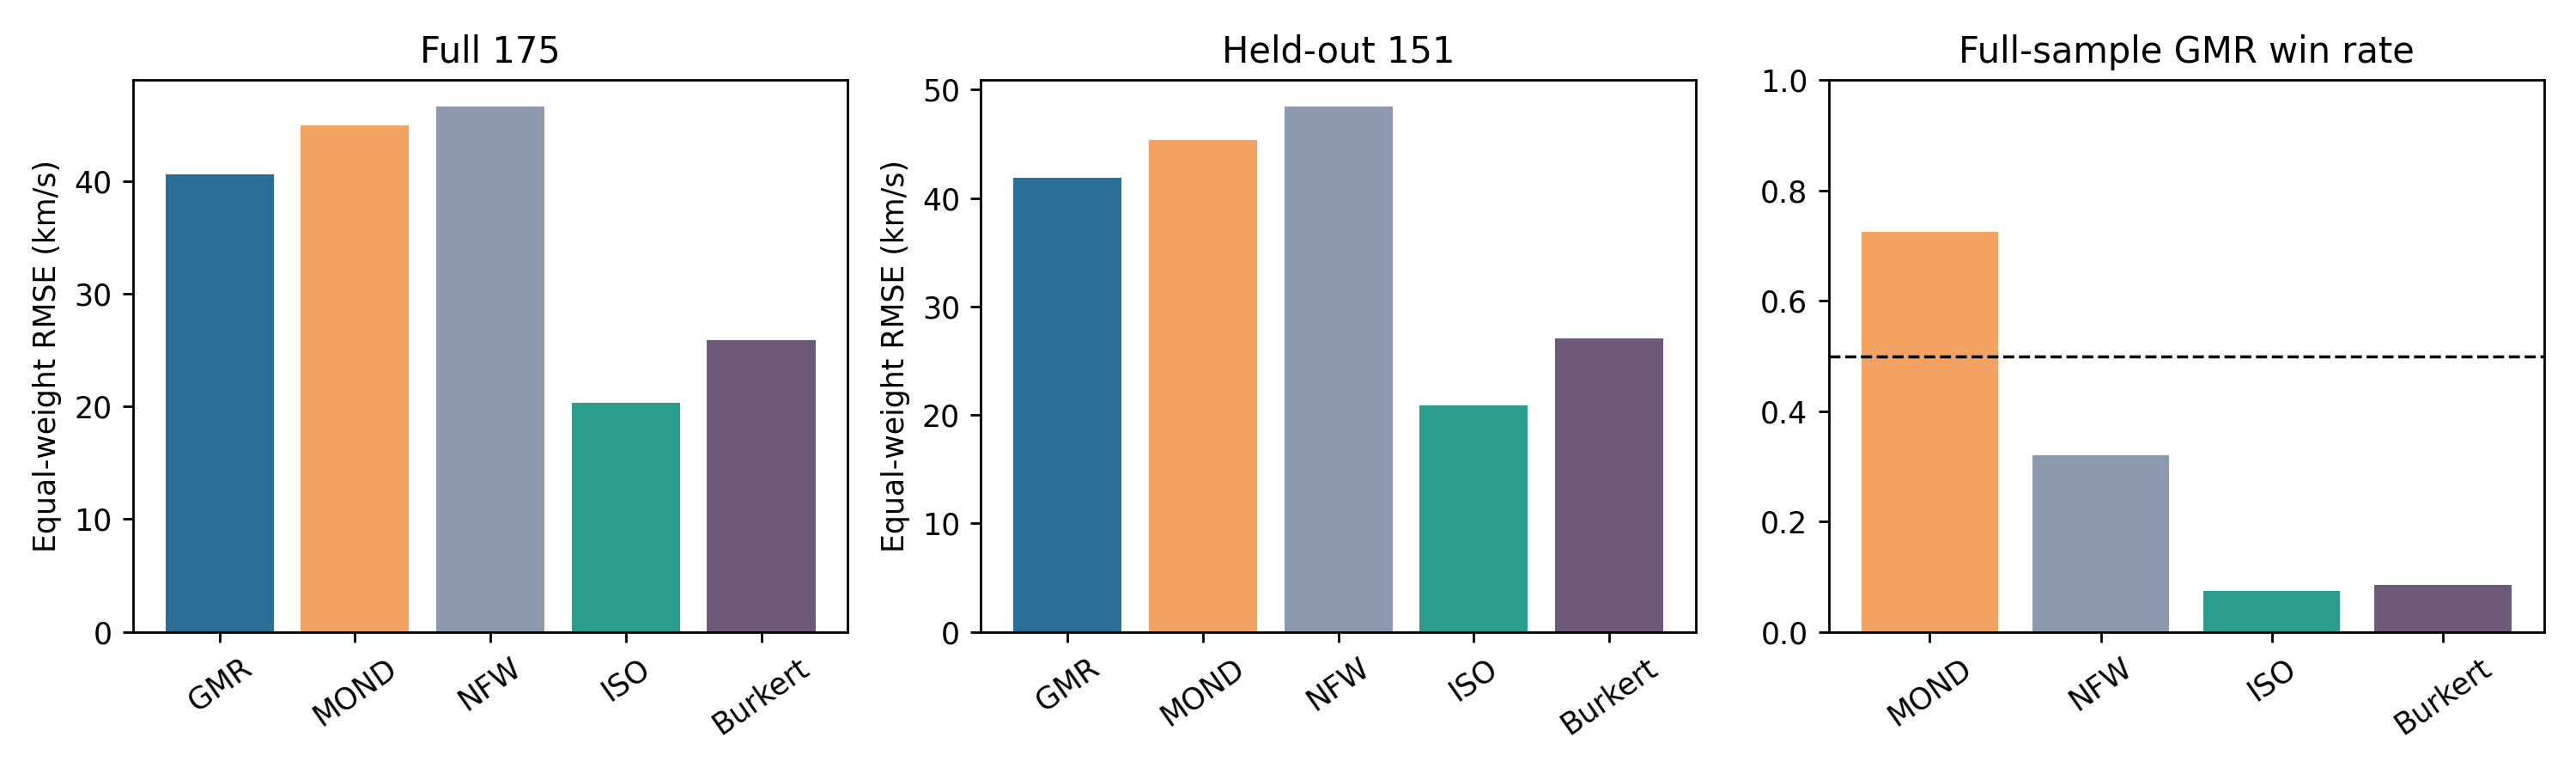
\includegraphics[width=0.48\textwidth]{figures/FIG2_metrics_comparison.png}
\caption{Summary of equal-weight RMSE for the original comparison set on the full 175-galaxy sample and held-out 151-galaxy subset, together with full-sample GMR win-rate diagnostics; the main table reports the pure square-root control immediately alongside the GMR rows. Mean, median, and additional win-rate caveats are tabulated in the text; this panel is not a complete multi-metric dominance plot. The pure square-root control baseline and local-$S_\Psi$ ablation are reported in the adjacent control-baseline rows of the aggregate RMSE table.}
\end{figure}

\begin{deluxetable*}{llrrrrl}
\tabletypesize{\scriptsize}
\tablecaption{Readable aggregate RMSE comparison, including control baselines and ablations. Negative $\Delta$ means lower aggregate RMSE for GMR; positive $\Delta$ means the comparator or control is lower. This table replaces compact slash notation so that the GMR value, comparator/control value, and caveat remain explicit.}
\tablehead{\colhead{Comparator} & \colhead{Sample} & \colhead{GMR RMSE} & \colhead{Comparator RMSE} & \colhead{$\Delta$RMSE} & \colhead{GMR WR} & \colhead{Caveat}}
\startdata
baryon & full & 40.554 & 69.316 & -28.762 & 0.886 & GMR lower RMSE \\
baryon & held-out & 41.870 & 71.026 & -29.156 & 0.874 & GMR lower RMSE \\
MOND & full & 40.554 & 44.907 & -4.353 & 0.726 & supportive, metric-dependent \\
MOND & held-out & 41.870 & 45.366 & -3.497 & 0.715 & supportive, metric-dependent \\
pure $\sqrt{g_N}$ baseline & full & 40.554 & 40.241 & +0.313 & \nodata & lower RMSE than GMR \\
pure $\sqrt{g_N}$ baseline & held-out & 41.870 & 41.329 & +0.541 & \nodata & lower RMSE than GMR \\
local-$S_\Psi$ variant & full & 40.554 & 47.683 & -7.129 & \nodata & local replacement worse \\
local-$S_\Psi$ variant & held-out & 41.870 & 49.398 & -7.528 & \nodata & cumulative state improves \\
reduced NFW & full & 40.554 & 46.613 & -6.059 & 0.320 & NFW wins median and win-rate \\
reduced NFW & held-out & 41.870 & 48.450 & -6.580 & 0.338 & NFW wins median and win-rate \\
reduced ISO & full & 40.554 & 20.316 & +20.238 & 0.074 & ISO stronger overall \\
reduced ISO & held-out & 41.870 & 20.869 & +21.001 & 0.079 & ISO stronger overall \\
reduced Burkert & full & 40.554 & 25.862 & +14.692 & 0.086 & Burkert stronger overall \\
reduced Burkert & held-out & 41.870 & 27.081 & +14.789 & 0.093 & Burkert stronger overall \\
\enddata
\end{deluxetable*}

\begin{deluxetable*}{llrrrr}
\tablecaption{Equal-weight and $N_{\rm obs}$-weighted RMSE diagnostics. The $N_{\rm obs}$-weighted diagnostic weights each galaxy by its number of rotation-curve points. It is descriptive and is not used to retune any model.}
\label{tab:nobs_weighted_rmse}
\tablehead{\colhead{Sample} & \colhead{Model} & \colhead{Equal-weight RMSE} & \colhead{$N_{\rm obs}$-weighted RMSE} & \colhead{EW rank} & \colhead{$N_{\rm obs}$ rank}}
\startdata
Full 175 & GMR & 40.554 & 57.334 & 3 & 4 \\
Full 175 & Baryons & 69.316 & 89.917 & 6 & 6 \\
Full 175 & MOND & 44.907 & 52.224 & 4 & 3 \\
Full 175 & NFW & 46.613 & 65.223 & 5 & 5 \\
Full 175 & ISO & 20.316 & 27.651 & 1 & 1 \\
Full 175 & Burkert & 25.862 & 37.664 & 2 & 2 \\
Held-out 151 & GMR & 41.870 & 61.586 & 3 & 4 \\
Held-out 151 & Baryons & 71.026 & 94.924 & 6 & 6 \\
Held-out 151 & MOND & 45.366 & 54.229 & 4 & 3 \\
Held-out 151 & NFW & 48.450 & 70.166 & 5 & 5 \\
Held-out 151 & ISO & 20.869 & 29.502 & 1 & 1 \\
Held-out 151 & Burkert & 27.081 & 40.827 & 2 & 2 \\
\enddata
\tablecomments{The rank inversion is important: on the $N_{\rm obs}$-weighted diagnostic MOND achieves a lower $N_{\rm obs}$-weighted RMSE than GMR, while ISO and Burkert remain stronger empirical halo baselines overall.}
\end{deluxetable*}

\section{Rotation-curve results}

All model comparisons in this section remain descriptive under the Holm-Bonferroni caveat in the statistical protocol. The central result is that the dominant SPARC aggregate signal is already captured by square-root scaling. The tested GMR invariant architecture organizes geometric departures from that scaling but does not improve the main RMSE benchmark. On the full 175-galaxy sample, GMR reaches an equal-weight RMSE of 40.554 km\,s$^{-1}$. The corresponding values for the comparators are 69.316 for baryons, 44.907 for MOND, 46.613 for reduced NFW, 20.316 for reduced ISO, and 25.862 for reduced Burkert. On the held-out 151-galaxy subset, the same ordering persists for the first four models: GMR records 41.870 against 71.026 for baryons, 45.366 for MOND, and 48.450 for reduced NFW, while reduced ISO and Burkert still sit at 20.869 and 27.081.

These aggregate numbers justify the narrow galaxy claim, but they do not by themselves tell the whole story. The rotation-curve panels are useful precisely because they expose how the aggregate statistic is assembled. In bulge-rich high-surface-brightness systems the implementation often tracks the overall shape well enough to produce large aggregate wins against baryons and visible advantages against MOND or reduced NFW. In ordinary disks the behavior is more mixed. Low-mass dwarfs are the clearest systematic weakness; a single visually acceptable dwarf panel does not overturn the class-level fact that the GMR-versus-reduced-NFW win rate is only 0.136 in the low-mass dwarf slice.

The main-text panels are therefore selected to represent both successful and challenging cases across the main morphology classes. They are chosen to show success and tension in each major morphology slice while excluding low-information curves with too few points. UGC02487 and UGC02885 illustrate that the implementation can perform credibly in bulge-rich and ordinary-disk systems without hidden retuning. NGC5371, UGC06930, and UGC07125 then show the kinds of residual tension that the analysis does not attempt to hide. One dwarf panel with tolerable agreement is retained for balance, but the interpretation of the dwarf regime is anchored to the class-level metrics rather than to a single example.

\begin{figure}[htbp]
\centering
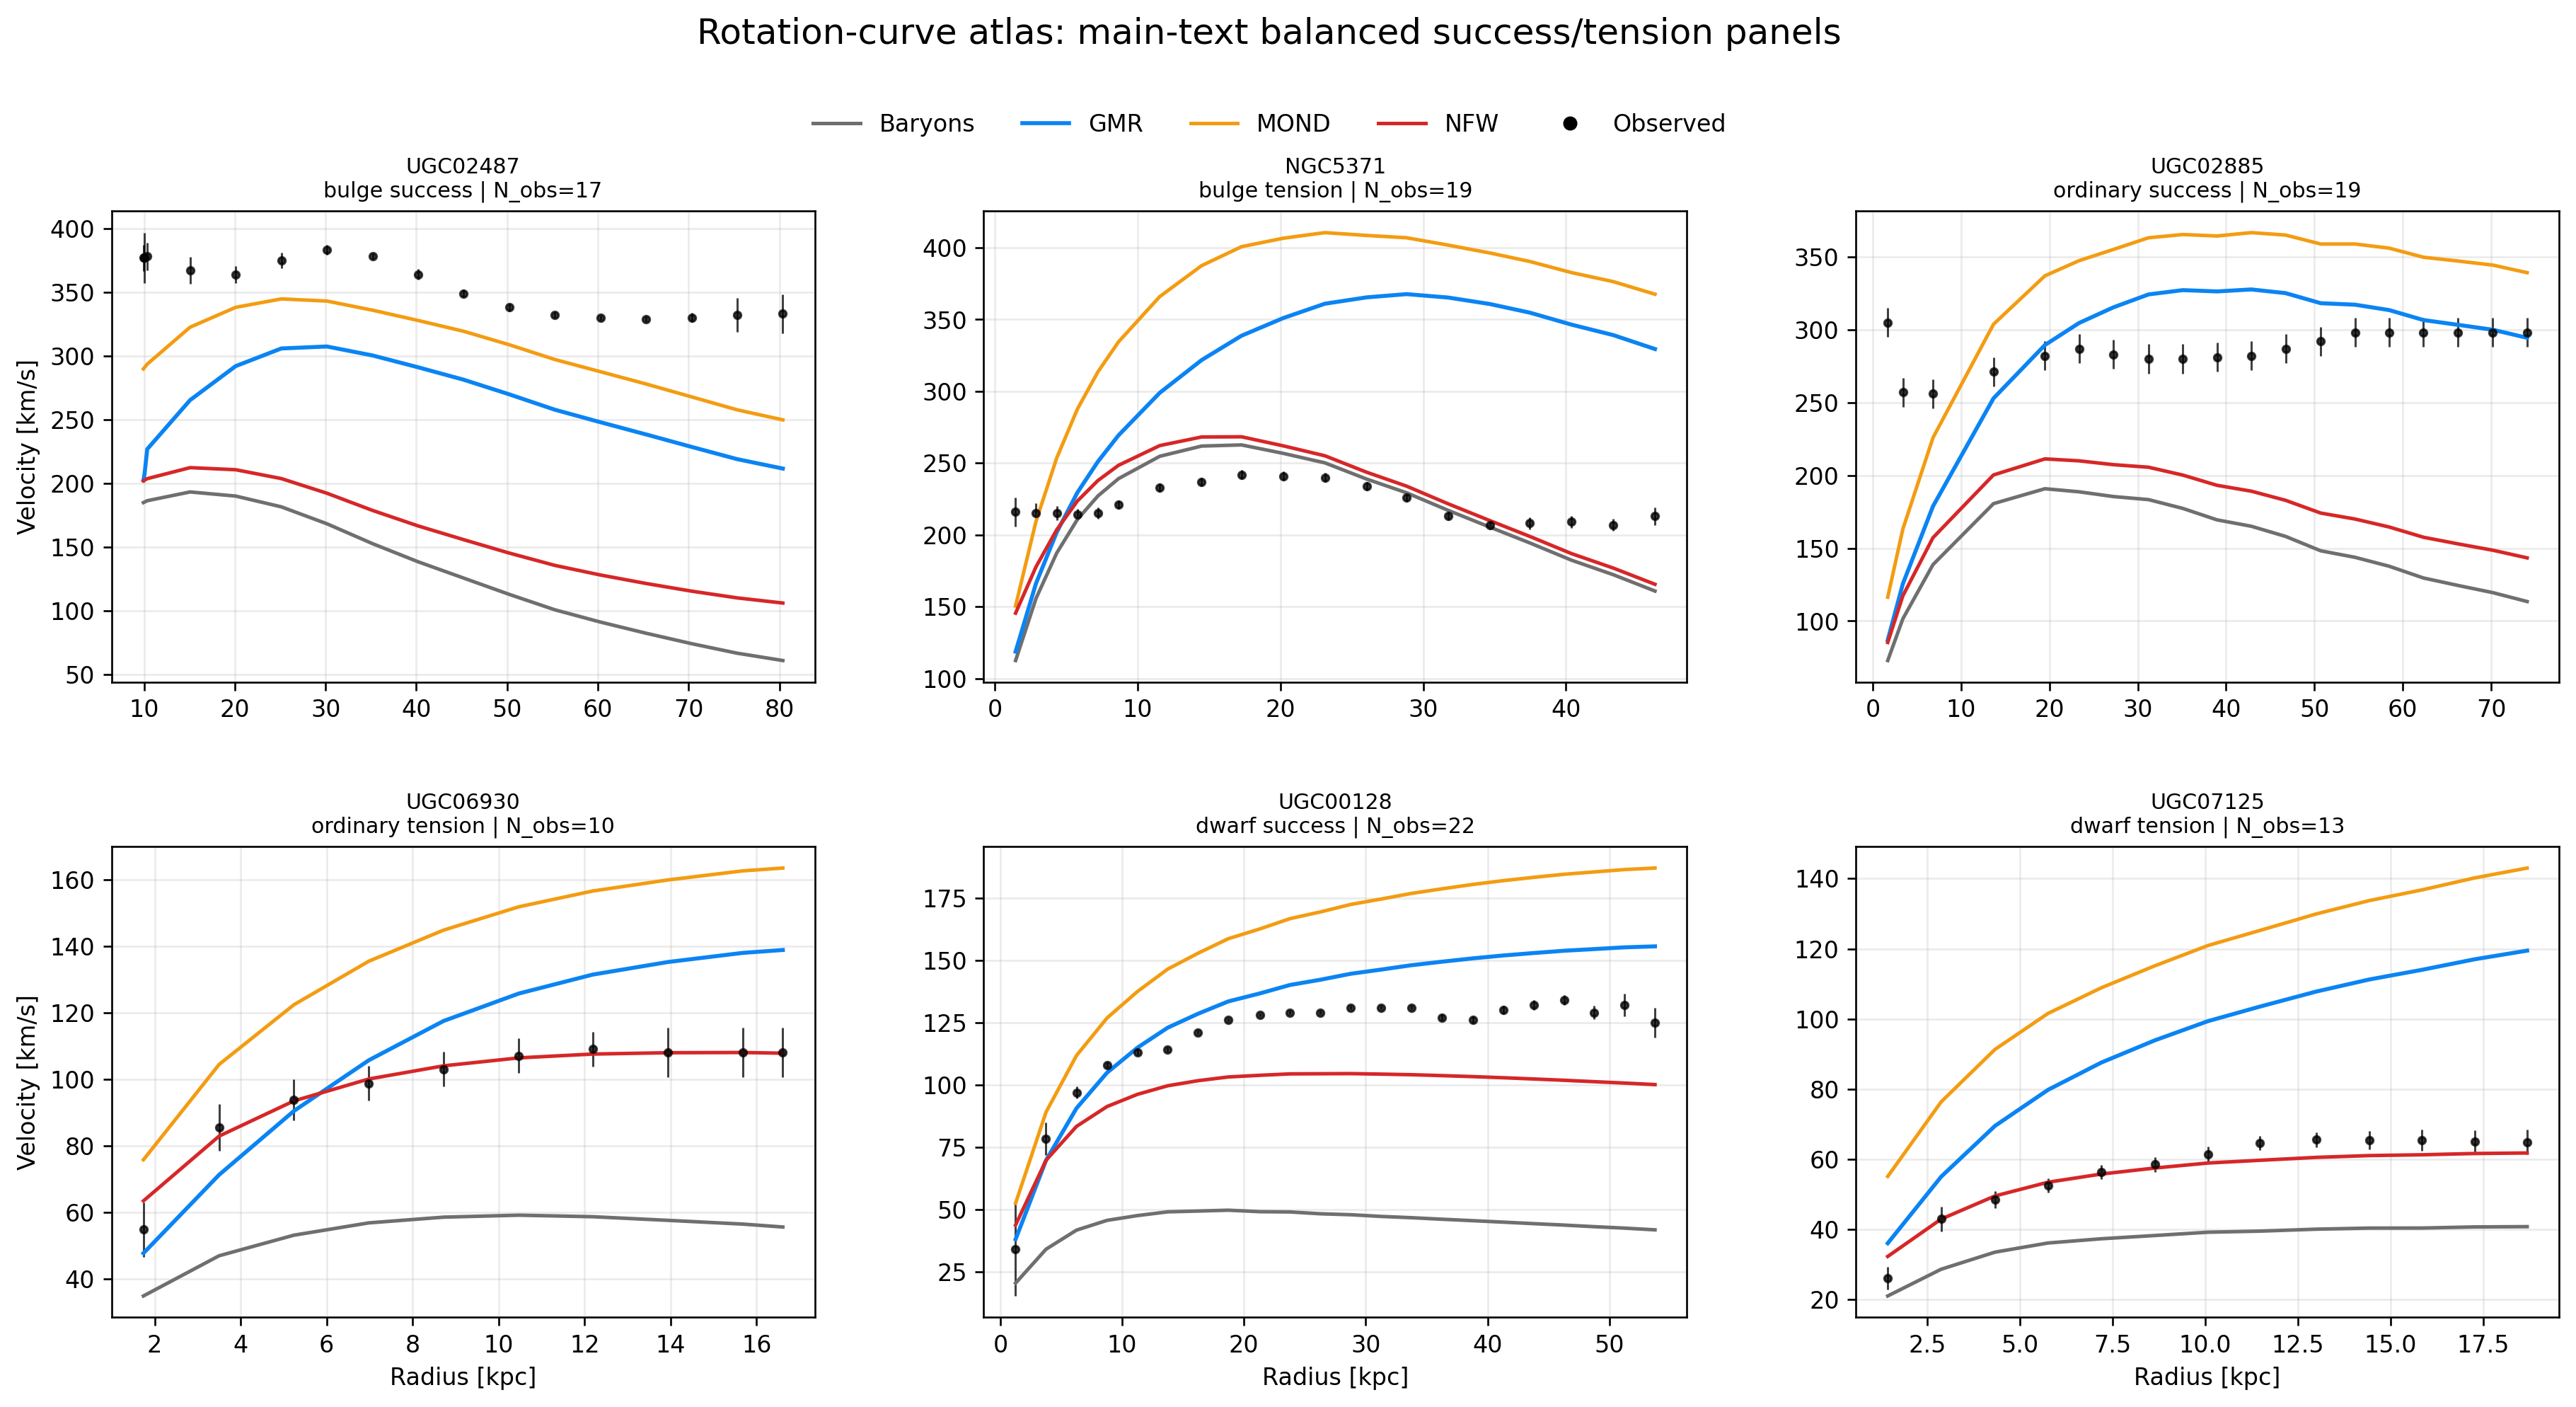
\includegraphics[width=0.48\textwidth]{figures/FIG1_rotation_curves.png}
\caption{Main-text rotation-curve panels. The six selected galaxies span bulge-rich success and tension cases, ordinary-disk success and tension cases, and dwarf-related context while respecting the minimum-information rule $N_{\rm obs}\ge 8$.}
\end{figure}

The extended atlas in the supplement continues this logic. It keeps gas-rich dwarf, diffuse dwarf, overall-best, and overall-worst panels available for transparency, but it does not overburden the main text. The figure split between main text and supplement is intended to help the reader identify the structure of the outcome rather than just a gallery of curves.
\section{Metric decomposition: RMS, mean, median, and win-rate}

The leverage decomposition in Figure~\ref{fig:leverage_by_galaxy} shows which galaxies drive the aggregate GMR--NFW mean-square difference. The top favorable systems are predominantly higher-surface-brightness or bulge-rich galaxies, whereas several bulge-rich tension cases work against the aggregate result. The source table is \texttt{tables/leverage\_by\_galaxy.csv}.

\begin{figure}[htbp]
\centering
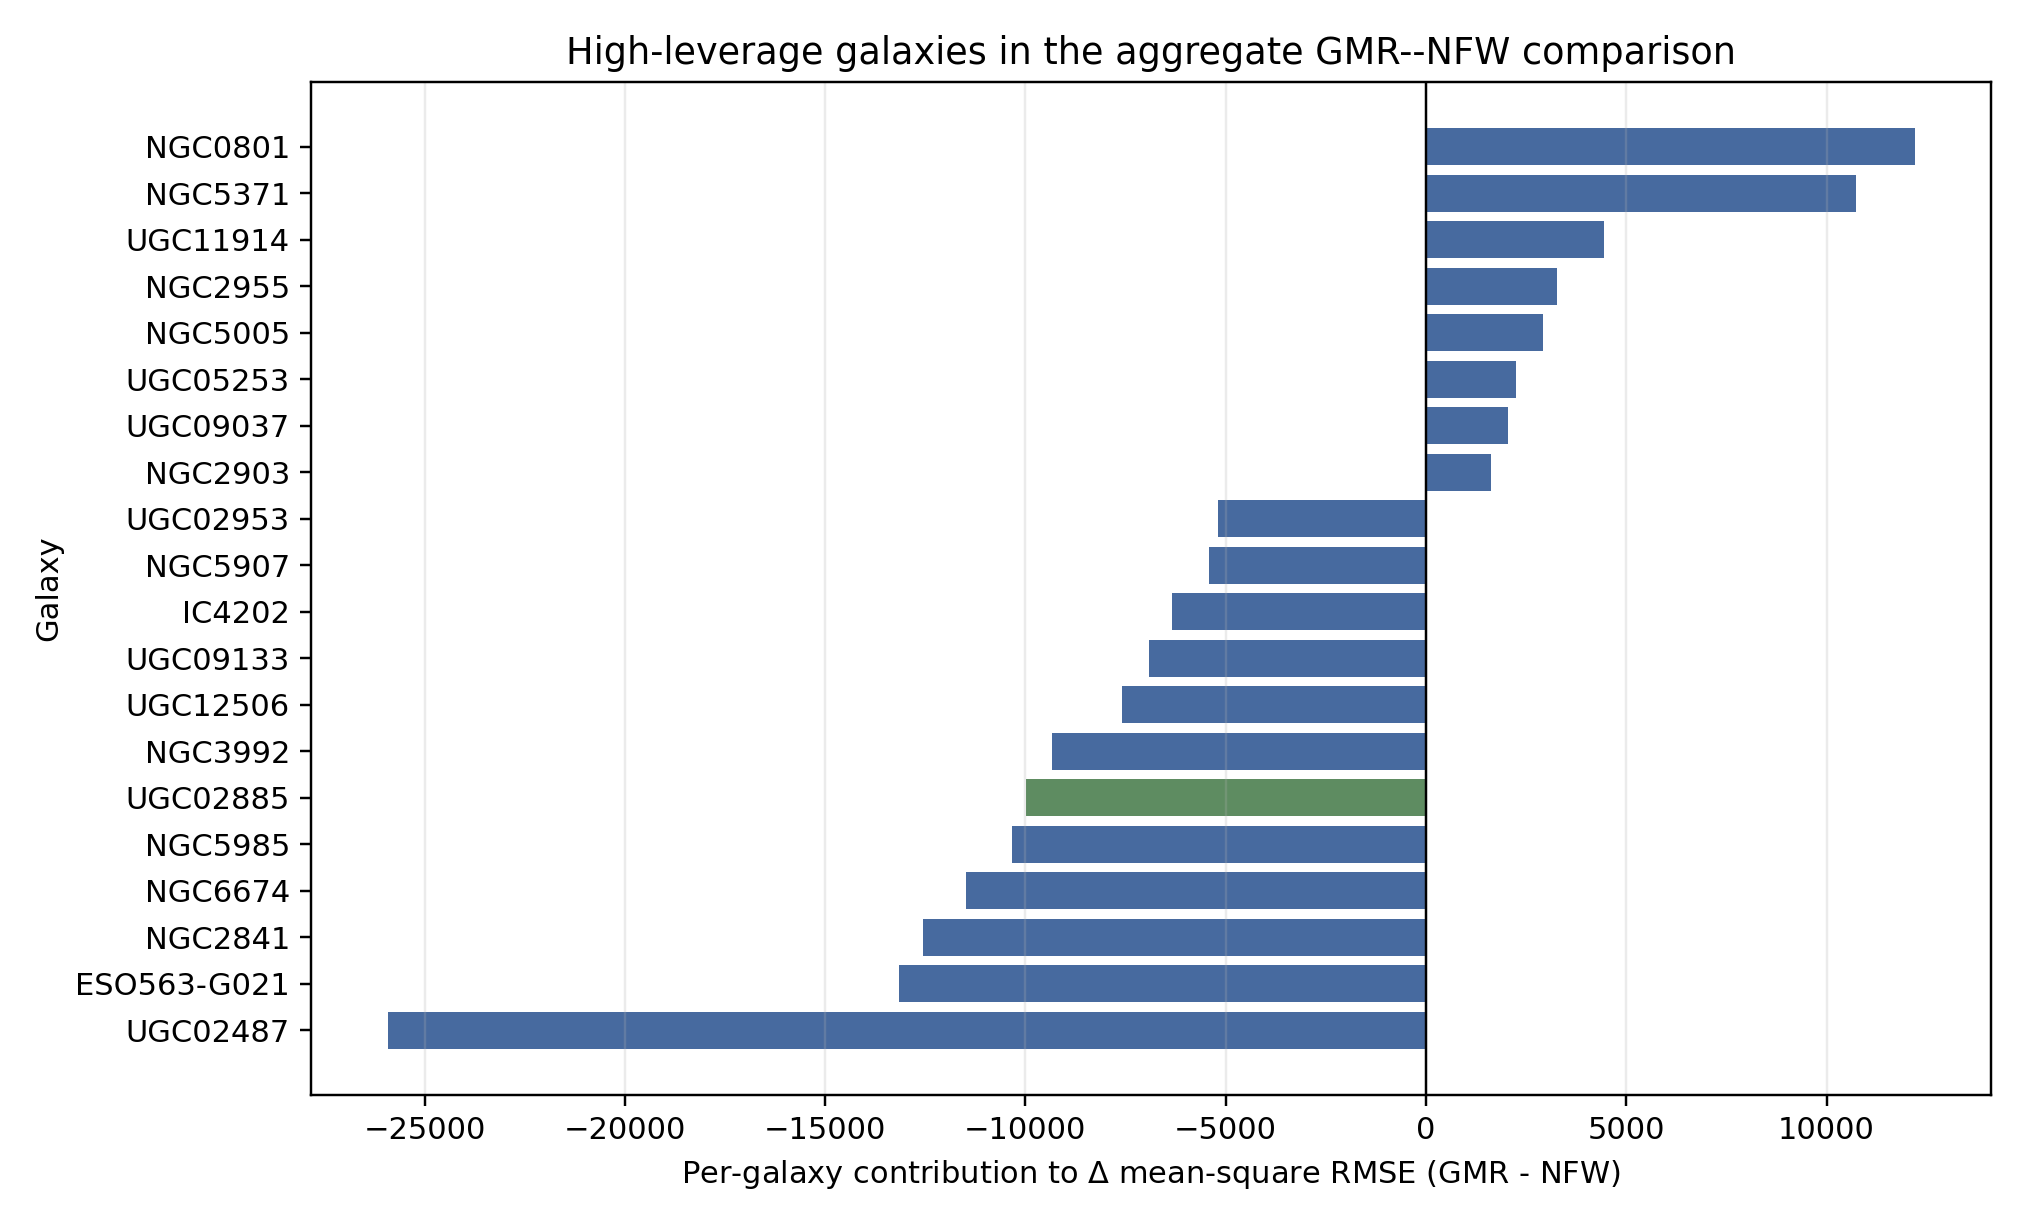
\includegraphics[width=0.48\textwidth]{figures/FIG7_leverage_by_galaxy.png}
\caption{High-leverage galaxy contributions to the aggregate GMR--NFW mean-square RMSE difference. Negative values favor GMR; positive values favor reduced NFW. The plot shows the largest favorable and unfavorable contributors, with colors denoting the morphology slice.}
\label{fig:leverage_by_galaxy}
\end{figure}

The decomposition across four metrics explains both why the analysis is scientifically useful and why it remains scope-limited. Against baryons, all four metrics line up in favor of GMR on both the full and held-out samples. Against MOND, the archived tables favor GMR on RMSE, mean absolute residual, median residual, and win rate as point estimates. That broad advantage is real, but the inferential support around the aggregate RMSE edge remains supportive rather than conventionally decisive: both the percentile and BCa interval checks retain a zero-crossing for at least the MOND comparison.

The reduced-NFW comparison is more nuanced and more central. On the full sample, GMR improves the equal-weight RMSE from 46.613 to 40.554 km\,s$^{-1}$ and improves the mean absolute residual from 25.319 to 24.073. Yet reduced NFW retains the smaller median residual, 7.048 against 13.349, and wins on 68\% of galaxies individually. The held-out subset tells the same story: GMR wins on equal-weight RMSE and mean absolute residual, but reduced NFW wins on median residual and on roughly 66\% of galaxies.

This illustrates how a single aggregate metric can misrepresent typical-galaxy performance when the improvement is concentrated in the tails of the residual distribution. The parameter-freedom asymmetry is part of the interpretation: GMR is a globally fixed response prescription, whereas the reduced halos are per-galaxy empirical baselines. A sentence of the form ``GMR beats NFW'' would be wrong, even though the aggregate RMSE result is real. The result indicates that GMR reduces the heavy tail of the reduced-NFW residual distribution more effectively than it improves the typical galaxy. The fixed response closure gains ground on the aggregate by avoiding some catastrophic failures, while reduced NFW still dominates local precision for the majority of systems.

The canonical bootstrap table reinforces that reading without over-selling it. For the full sample, the delta equal-weight RMSE is -6.059 km\,s$^{-1}$ against reduced NFW, with a 95\% interval [-11.444, -0.728] and a bootstrap-negative fraction of 0.987. On the held-out subset, the corresponding values are -6.580, [-12.538, -0.550], and 0.985. Those numbers support a real aggregate edge while leaving the median and win-rate caveats fully visible.

\begin{figure}[htbp]
\centering
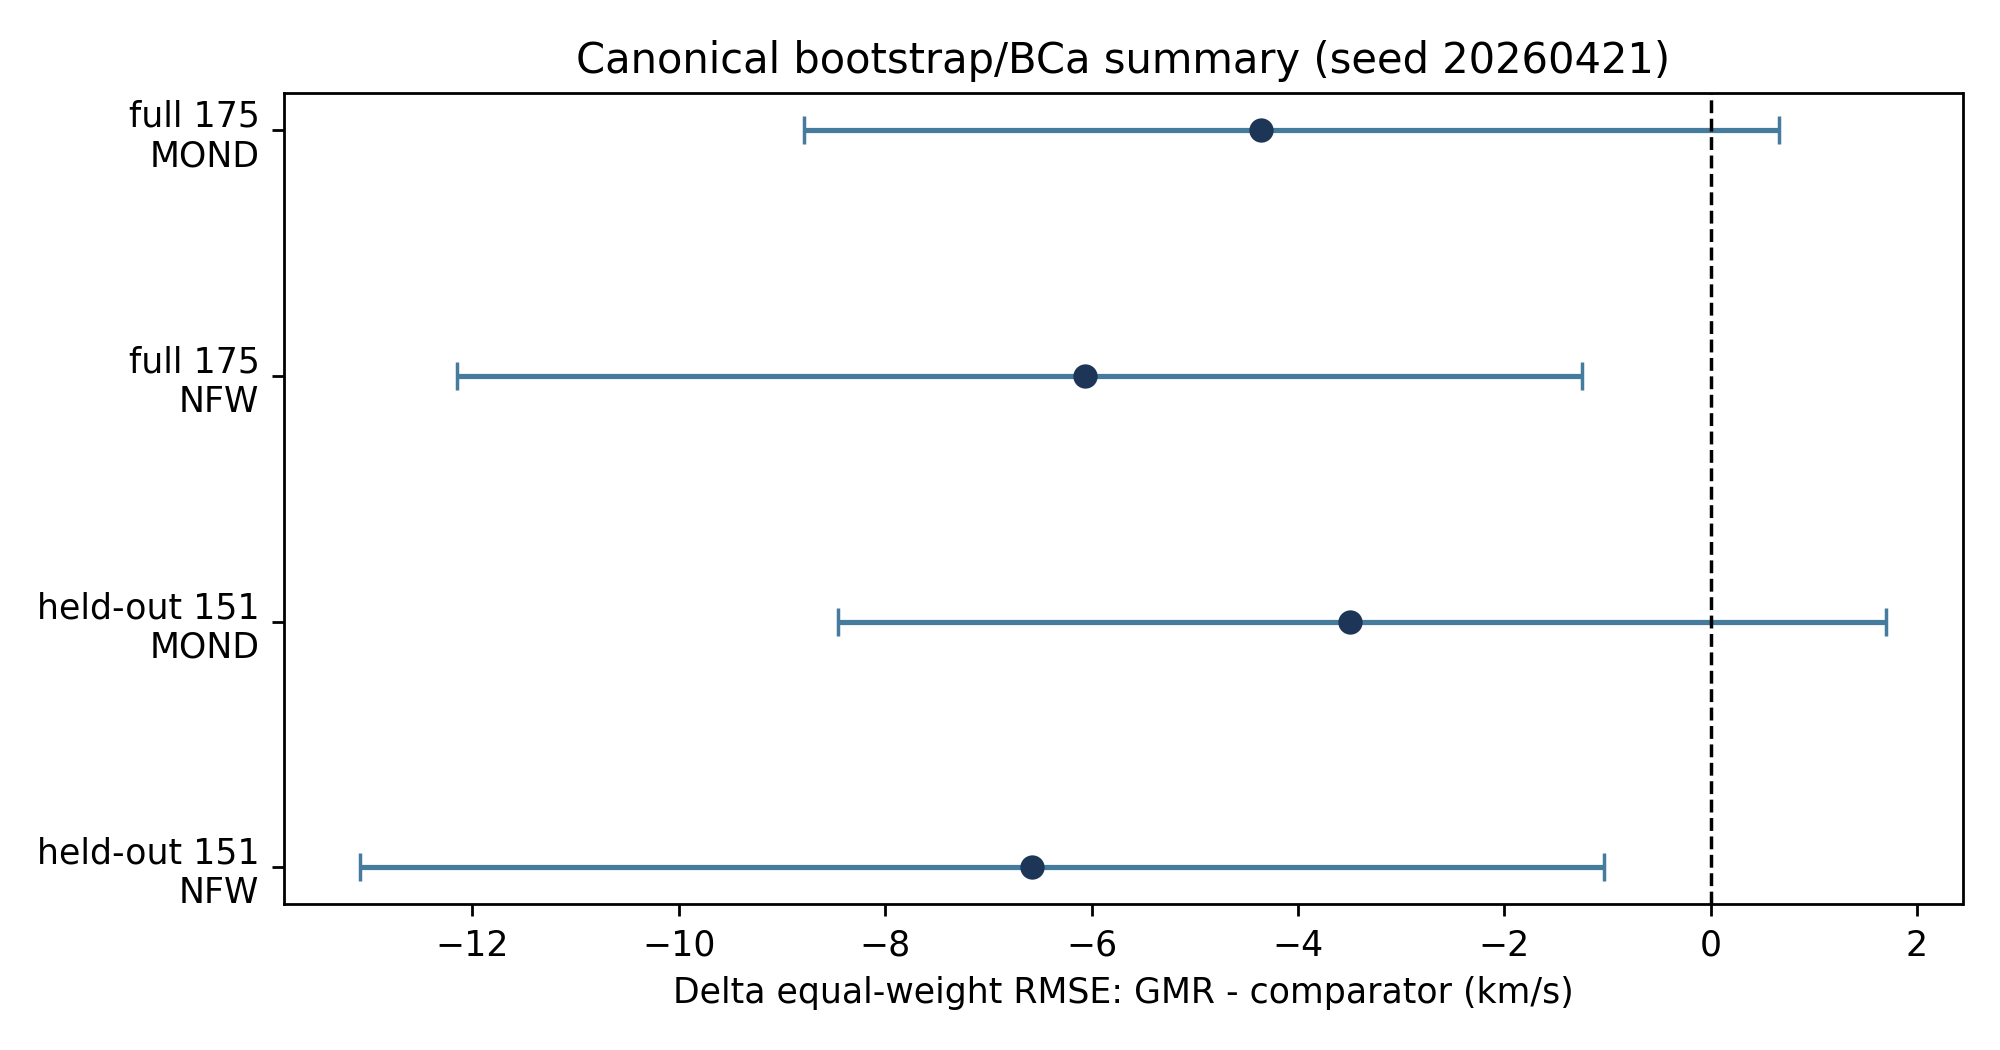
\includegraphics[width=0.48\textwidth]{figures/FIG5_bootstrap_summary.png}
\caption{Bootstrap delta-RMSE summary for the full and held-out samples against MOND and reduced NFW. The MOND intervals still overlap zero, whereas the reduced-NFW intervals remain negative.}
\end{figure}

The outlier and leave-class-out diagnostics refine the picture further. On the held-out subset, removing the nine most favorable galaxies to GMR is enough to reverse the aggregate sign against both MOND and reduced NFW. That does not invalidate the aggregate result, but it means the advantage is partly driven by a finite set of high-leverage successes. Leave-class-out tests show that the reduced-NFW comparison depends strongly on bulge-rich high-surface-brightness systems. The paper therefore treats the aggregate result as real but morphology-structured.
\section{RAR consistency}

The radial-acceleration relation remains one of the strongest diagnostics in the machine-readable analysis tables. Using the archived binned RAR products carried in the final tables, the study recomputes a log-space RMSE of 0.0640 for GMR against the official binned target, compared with 0.2032 for the MOND baseline used in the same fixed product. The archived RAR products use 13 equal-weight stored binned residual rows for the GMR and MOND binned series over log $g$ range -11.69 to -9.12; official comparison bins are stored separately in \texttt{rar\_binning\_spec.csv}.

The interpretation of that number is intentionally narrow. Because the fixed global amplitude was calibrated on a SPARC subset, the RAR is not presented here as an independent validation set. Instead, it is a within-sample consistency diagnostic: it shows that the same fixed implementation that produces the rotation-curve metrics also tracks the archived binned acceleration relation more closely than the corresponding MOND baseline in the same analysis products.

That narrower framing keeps the RAR useful without letting it do too much rhetorical work. The result is still scientifically interesting because it compresses thousands of kinematic points into an acceleration-space diagnostic and shows that the fixed GMR prescription captures more than one summary statistic. But the manuscript does not use the RAR as a substitute for the rotation-curve caveats or as a claim of independent validation.

\begin{figure}[htbp]
\centering
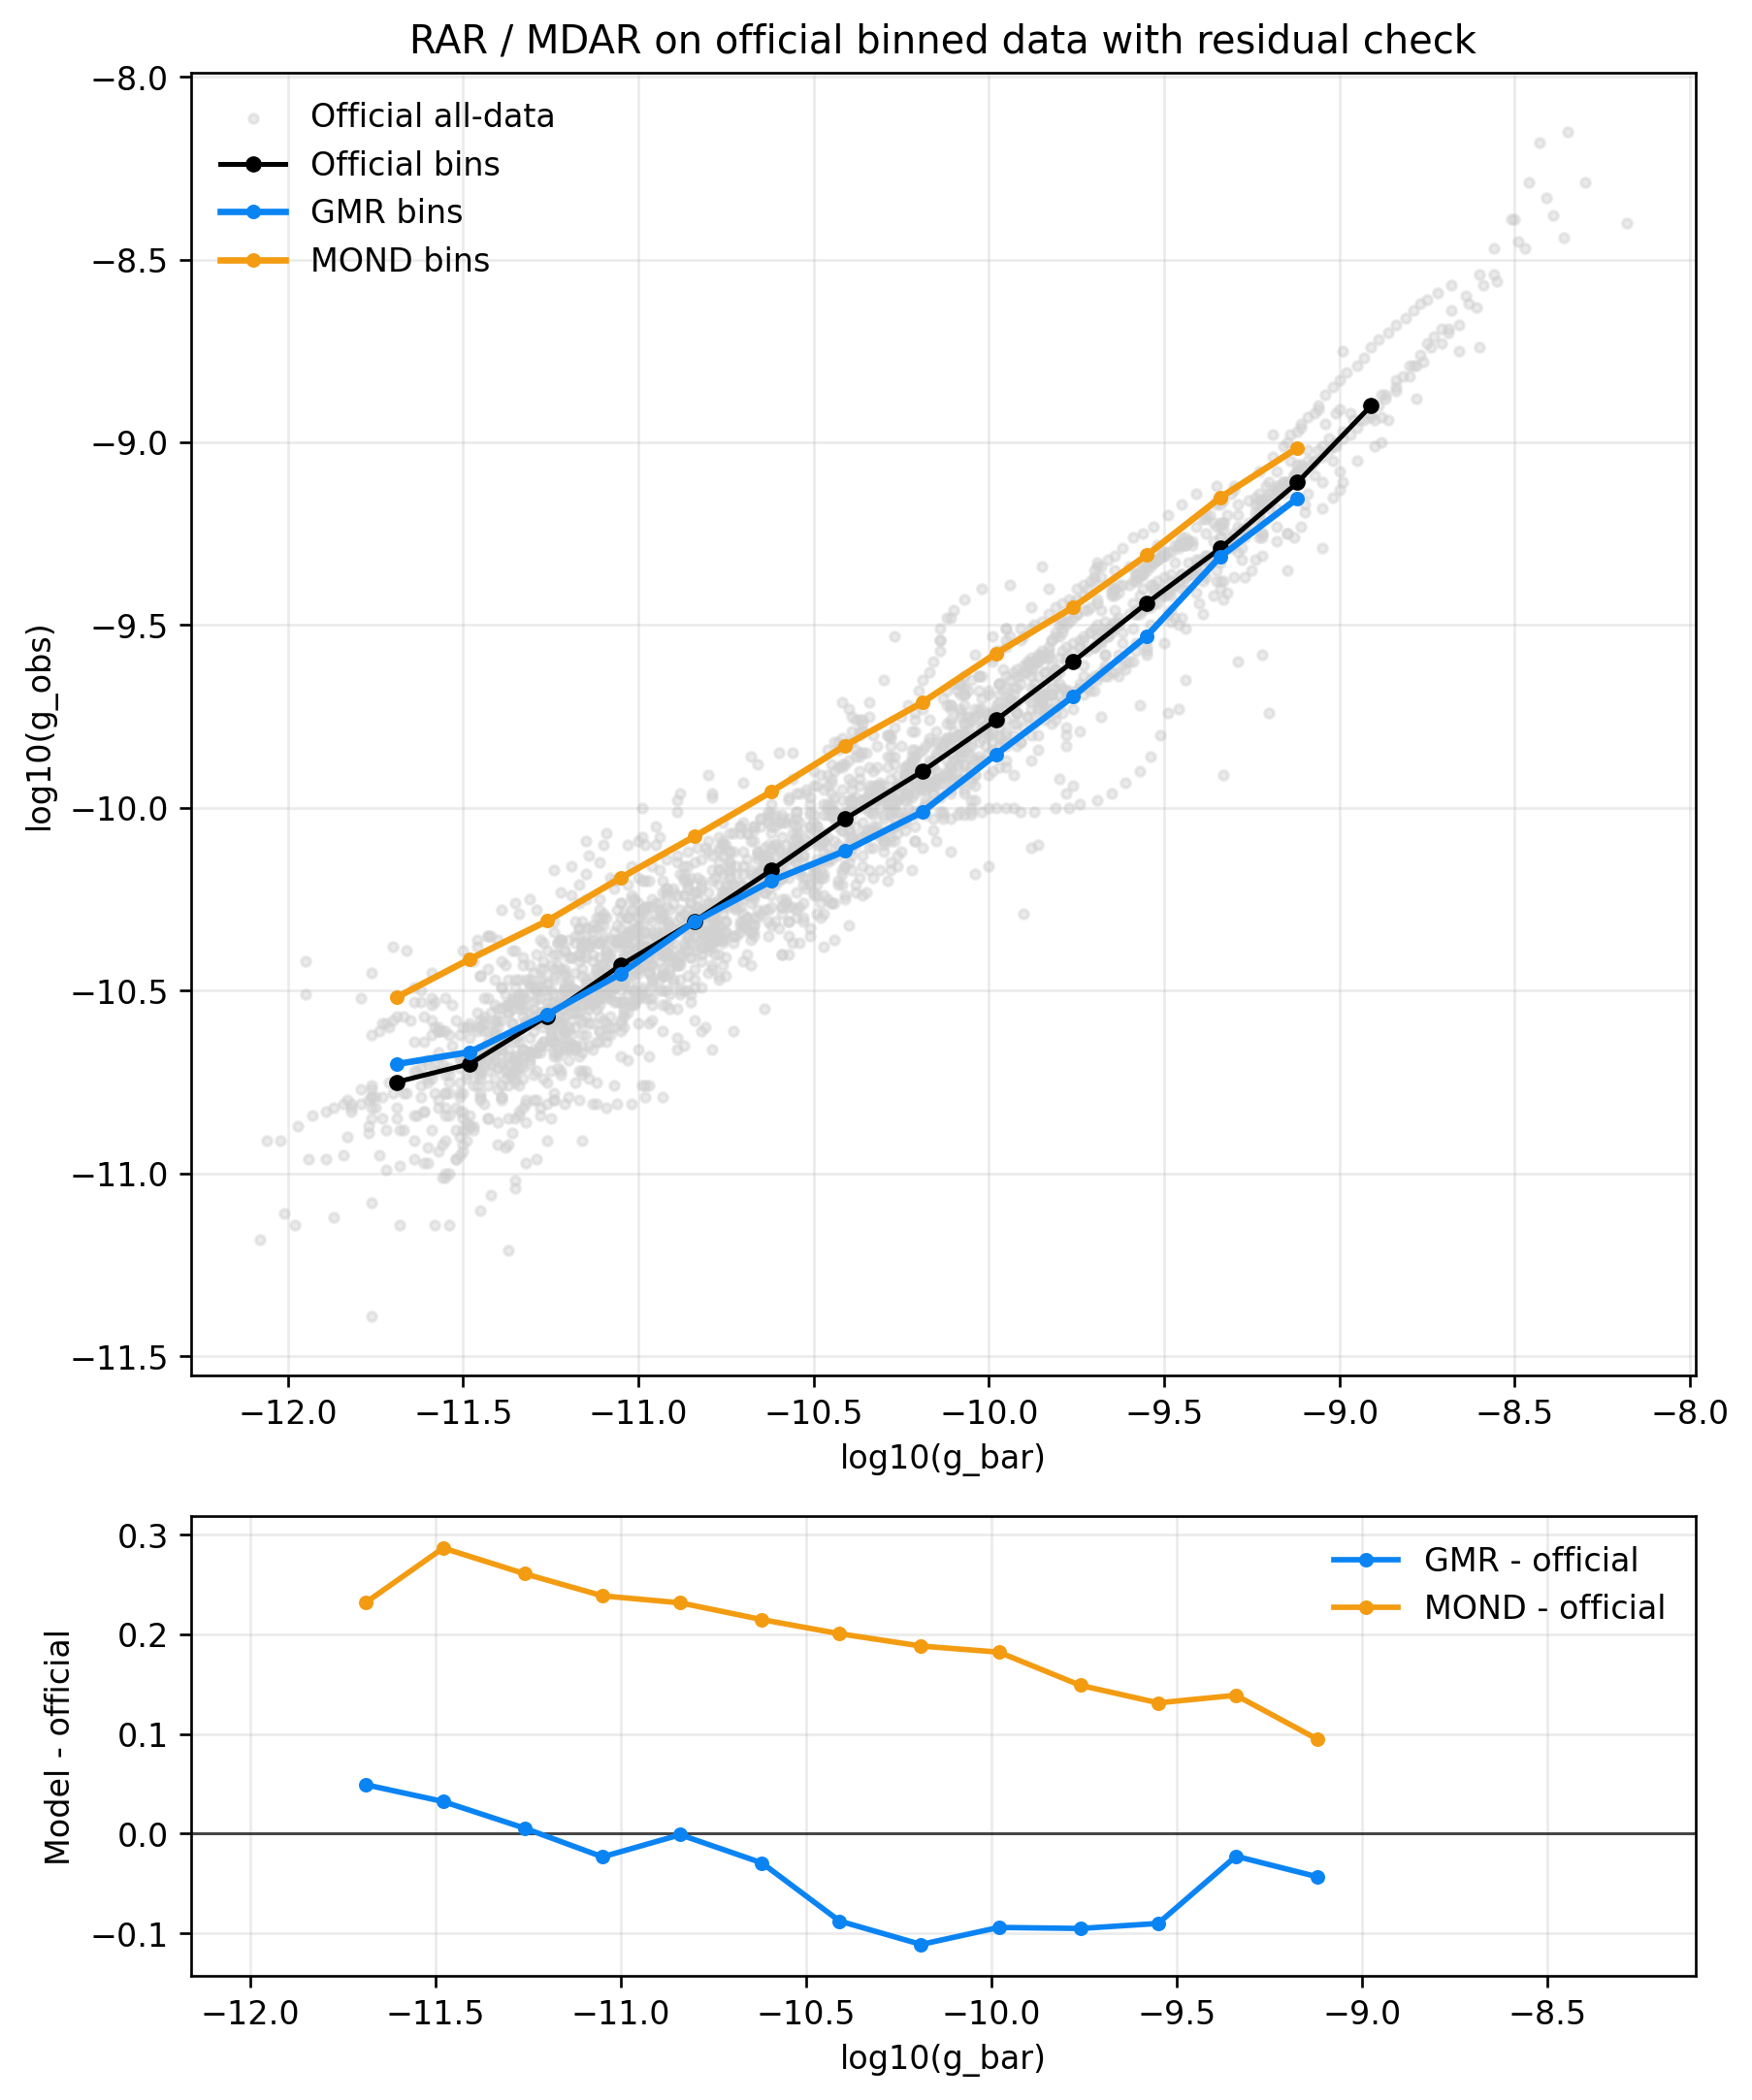
\includegraphics[width=0.48\textwidth]{figures/FIG3_RAR.png}
\caption{Binned radial-acceleration relation comparison using the fixed study machine-readable RAR products. It is interpreted here as a within-sample consistency diagnostic, not as an independent validation set.}
\end{figure}
\section{BTFR consistency}

The baryonic Tully-Fisher relation plays a complementary role. It is not the main discovery claim of the paper, but it is a useful scaling-law check on whether the fixed proxy preserves a sensible relation between baryonic mass and rotational scale. The machine-readable fit summaries carried in the final analysis give an observed slope of 3.486 and a fixed GMR proxy slope of 3.687. The observed scatter is 0.225 dex, while the fixed GMR proxy scatter is 0.285 dex.

The correct reading is therefore ``slope-consistent with broader scatter.'' That sentence is intentionally modest. The slope difference is small enough that the proxy sits in the same broad BTFR family, but the broader scatter means the fixed implementation does not reproduce the tightness of the observed relation. The BTFR is therefore supportive rather than decisive.

\begin{figure}[htbp]
\centering
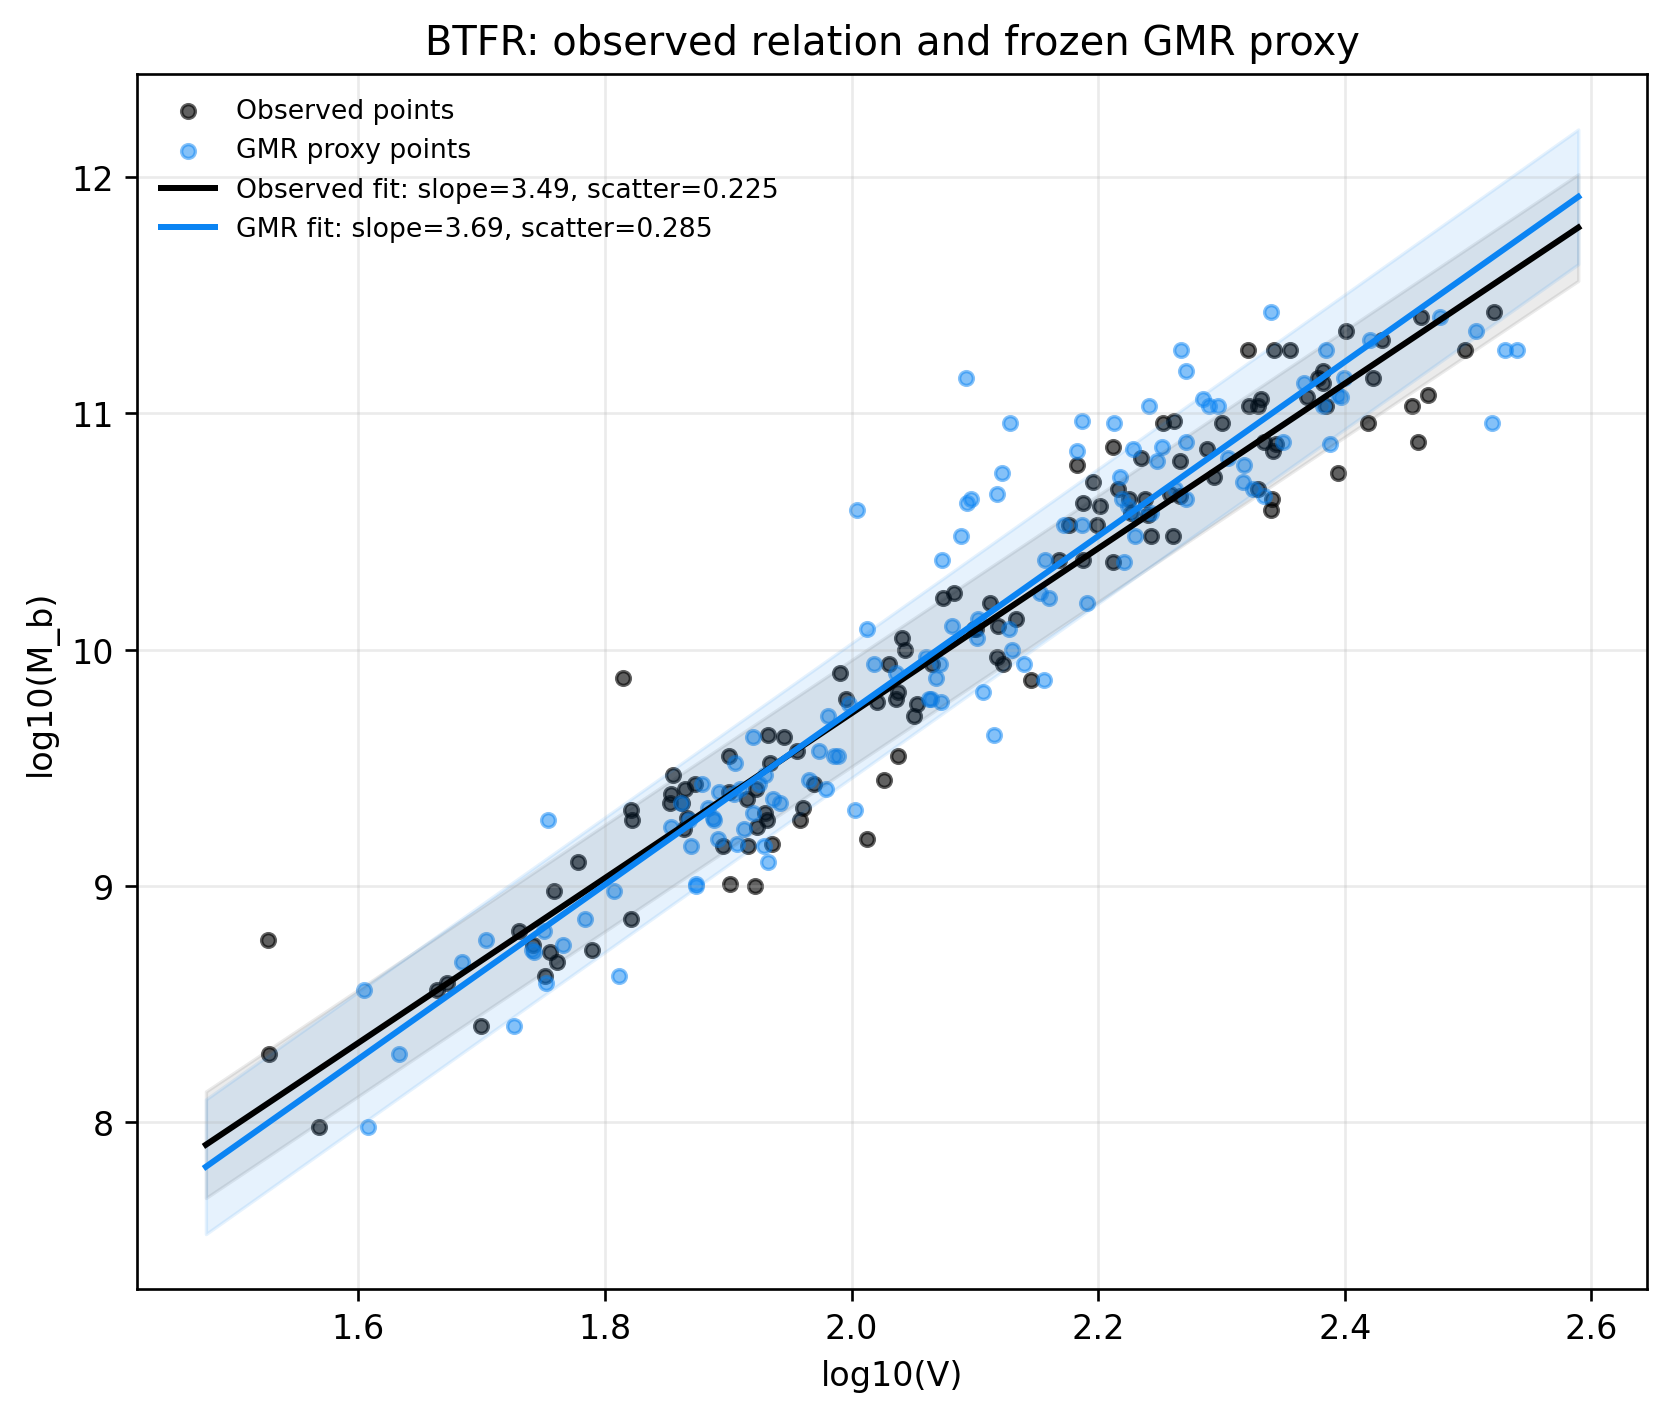
\includegraphics[width=0.48\textwidth]{figures/FIG4_BTFR.png}
\caption{Baryonic Tully-Fisher relation comparison using the fixed GMR proxy velocity against the observed SPARC flat-velocity compilation. The fit remains slope-consistent but broader in scatter than the observed relation.}
\end{figure}
\section{Failure modes: diffuse dwarfs, low-surface-brightness systems, and ordinary disks}

The main empirical limitation of GMR is now stated as plainly as possible. Low-mass, low-surface-brightness, gas-rich dwarf systems are the clearest systematic weakness of the fixed implementation. In the stratified stress table, the low-mass-dwarf class reaches an equal-weight RMSE of 15.523 for GMR against 6.880 for reduced NFW and 4.478 for reduced ISO, with a GMR-versus-reduced-NFW win rate of only 0.136. Ordinary disks are intermediate but still problematic.

The correlation diagnostics point in the same direction. Lower effective surface brightness correlates with larger GMR-minus-NFW failure, while gas fraction correlates positively with failure and total luminosity correlates negatively. These are not perfect one-parameter explanations, but they are strong enough to justify the paper's emphasis on low-density and gas-rich regimes.

At the same time, the top-failure list cautions against an overly simple narrative. The largest individual failures include low-mass-dwarf systems such as F574-2 and UGC07125, but also bulge-rich galaxies such as NGC5371 and NGC0801. The paper therefore speaks of the \emph{principal empirical tension} being in the diffuse-dwarf, low-surface-brightness, and ordinary-disk sector rather than claiming that every bad case lives there.

\begin{deluxetable}{lrrrrr}
\tablecaption{Stratified class-level stress test on the fixed full 175-galaxy benchmark.}
\tablehead{\colhead{Class} & \colhead{N} & \colhead{GMR RMSE} & \colhead{MOND RMSE} & \colhead{NFW RMSE} & \colhead{GMR vs NFW win-rate}}
\startdata
bulge\_rich\_hsb & 77 & 58.080 & 59.306 & 68.390 & 0.532 \\
low\_mass\_dwarf & 81 & 15.523 & 27.778 & 6.880 & 0.136 \\
ordinary\_disk & 17 & 22.428 & 33.944 & 30.933 & 0.235 \\
\enddata
\end{deluxetable}

Top-failure summary: NGC5371 (bulge-rich HSB, GMR minus NFW 79.292); NGC0801 (bulge-rich HSB, GMR minus NFW 69.282); F574-2 (low-mass dwarf, GMR minus NFW 35.595); UGC07125 (low-mass dwarf, GMR minus NFW 34.273); UGC06628 (low-mass dwarf, GMR minus NFW 31.975); UGC09037 (bulge-rich HSB, GMR minus NFW 29.947).

The leave-class-out results reinforce the same lesson. Excluding low-mass dwarfs does not erase the aggregate comparison, but excluding bulge-rich high-surface-brightness galaxies removes much of the model's leverage against reduced NFW. In other words, the aggregate success depends heavily on where the fixed prescription performs best, while its systematic weakness remains concentrated in low-density classes. This pattern is reported explicitly because it affects how the aggregate result is interpreted.
\section{Discussion}

\paragraph{Recovered radial diagnostics included in the public release.} The recovered radial diagnostics contain 3391 radial points for all 175 galaxies and include the tabulated and plotted $\sin\alpha_B S_{\rm rad}$ factor, a pure $\sqrt{g_N}$ baseline optimized on \texttt{calibration\_24}, and a local-$S_\Psi=\nu_B/(1+\nu_B)$ variant. The pure globally fitted square-root response baseline reaches a slightly lower equal-weight RMSE than the full GMR prescription on both the full and held-out samples. The dominant SPARC aggregate signal is therefore already captured by square-root scaling. The tested GMR invariant architecture organizes geometric departures from that scaling but does not improve the main RMSE benchmark. The local-$S_\Psi$ replacement gives equal-weight RMSE 47.683 km\,s$^{-1}$ on the full sample and 49.398 km\,s$^{-1}$ on the held-out subset, so the cumulative state variable improves over this tested local replacement. This negative/constraint result is scientifically useful: it shows that the tested local tidal/compactness invariants, even with a cumulative state variable, are insufficient to outperform the simpler square-root response on the present SPARC aggregate metric.


The fixed GMR configuration is interpreted as a fixed, scope-limited phenomenology for disk-galaxy rotation curves. Its strongest result is not superiority over the square-root control, but the reproducible constraint that the tested geometric invariant structure does not improve the main aggregate benchmark beyond that simpler response. The improvement is concentrated in the equal-weight aggregate RMSE and should not be interpreted as typical-galaxy superiority. Reduced NFW retains the median-residual and per-galaxy win-rate advantage. Reduced ISO and Burkert remain stronger empirical halo baselines overall.

That combination of strengths and weaknesses is scientifically informative. The model performs best in bulge-rich high-surface-brightness systems and worst, in a systematic sense, in low-density, gas-rich, and low-mass regimes. The low-mass, low-surface-brightness dwarf regime is the main empirical failure mode of the present GMR prescription. This suggests that the present cumulative state variable and suppression factor do not yet capture the response structure of low-density, gas-rich systems. The top-failure list shows that a few large outliers also occur in bulge-rich galaxies, so the low-density diagnosis is best understood as the principal empirical tension rather than an exclusive one.

The held-out equal-weight RMSE is reported as the main descriptive aggregate metric; mean, median, win rate, RAR, BTFR, and the stratified diagnostics are descriptive diagnostic quantities. The narrow empirical statement is therefore a constraint on the added value of the tested invariant architecture, not a claim of fitting-model dominance. It also clarifies why the reduced-NFW comparison remains interesting even though GMR loses on local precision for most galaxies: the question is whether a fixed response prescription can carry a nontrivial aggregate signal, not whether it beats a flexible per-galaxy halo fit on every lens. A matched global-halo baseline, such as an NFW concentration--mass scaling relation or another low-dimensional halo scaling prescription, is not implemented here and remains an important next comparator. Therefore, the present results should not be read as broad superiority over dark-matter halo prescriptions generally.

A separate theoretical program may eventually try to address action-based closure, local screening, cosmology, or strong-field behavior. This analysis does not. Its contribution is narrower and more defensible: a fixed SPARC rotation-curve phenomenology with explicit caveats, transparent failure modes, and reproducibility artifacts aligned to the machine-readable tables.
\section{Conclusions}

The present results support a narrow but non-trivial constraint. On the official SPARC benchmark, a pure square-root response slightly outperforms the fixed GMR implementation on the aggregate equal-weight RMSE metric, even though GMR remains globally specified and competitive relative to baryons-only, MOND, and reduced NFW. The full and held-out benchmark values are 40.554 and 41.870 km\,s$^{-1}$ for GMR, compared with 44.907/45.366 for MOND and 46.613/48.450 for reduced NFW. However, the pure globally fitted square-root response baseline reaches 40.241 and 41.329 km\,s$^{-1}$ on the same full and held-out aggregate metric. The present results therefore do not establish that the full baryonic-invariant GMR architecture improves over a simpler square-root response on the main descriptive aggregate metric.

This does not imply blanket superiority. Reduced NFW retains the smaller median residual and the higher per-galaxy win rate, and reduced ISO and Burkert remain stronger empirical halo baselines overall. The principal empirical limitation of the current implementation occurs in low-mass, low-surface-brightness dwarf systems, where flexible halo descriptions retain a marked local advantage.

The appropriate interpretation is therefore phenomenological rather than total-theoretical. GMR provides a reproducible galaxy-scale response test on SPARC without galaxy-by-galaxy retuning, but the present benchmark shows that its tested baryonic-invariant structure is not yet empirically required beyond square-root scaling. Screening, cosmological closure, clusters, and strong-field behavior remain outside the scope of the present paper. Within that deliberately restricted scope, the main contribution of this work is to provide a falsifiable public constraint on which parts of the geometric-medium response framework are, and are not, supported by the present rotation-curve benchmark.





 \begin{acknowledgments}
The author acknowledges the use of the SPARC database and thanks the developers and maintainers of the public astronomical resources used in this work. The author also acknowledges the use of NASA's Astrophysics Data System. The author acknowledges institutional support from the Faculty of Sciences, Belhadj Bouchaib University of Ain Temouchent. This research received no external funding.

\software{Python, NumPy, pandas, SciPy, Matplotlib}
\end{acknowledgments}
\section{Data and software availability}

The SPARC input data are publicly available from the SPARC database. The derived analysis products and code, including the recovered radial-input tables \texttt{full\_radial\_invariants.csv} and \texttt{all\_galaxy\_radial\_predictions.csv}, are prepared for public archiving; the repository URL and archive DOI will be inserted before journal upload.

\bibliographystyle{aasjournalv7}
 \bibliography{references_v55}
 \end{document}
